\section{Première formulation robuste}
\subsection{Modèle}
Afin de prendre en compte les erreurs sur les facteurs d'amplification $x_i$, nous utilisons les valeurs maximales des variations possibles de $\hat{D(\theta)}$ sur un intervalle.\\
\begin{eqnarray}
|\hat{D(\theta)}| & = & |\sum_{i=1}^{n} x_i(1+\xi_i)d_i(\theta)| \nonumber \\
& \leq & |\sum_{i=1}^{n} x_i d_i(\theta)| + |\sum_{i=1}^{n} x_i \xi_i d_i(\theta)| \nonumber \\
& \leq & |D(\theta)| + \sum_{i=1}^{n} |\tau d_i(\theta)\frac{h}{2}| \nonumber
\end{eqnarray}
En imposant 
$$|D(\theta)| + \sum_{i=1}^{n} |\tau d_i(\theta)\frac{h}{2}|\leq \epsilon $$
on est sur que $|\hat{D(\theta)}|\leq \epsilon$. De la même manière, on traduit les contraintes sur P : 
$$|D(\theta)-1| + \sum_{i=1}^{n} |\tau d_i(\theta)\frac{h}{2}|\leq \epsilon $$
Il nous faut donc introduire n variables $v_i$ pour chaque $\theta$ échantillonné, correspondant aux valeurs absolues des $\tau d_i(\theta)\frac{h}{2}$
On a alors 
\begin{eqnarray}
|D(\theta)| + \sum_{i=1}^{n} |\tau x_i d_i(\theta)\frac{h}{2}| & \leq & \epsilon \nonumber \\
|D(\theta)-1| + \sum_{i=1}^{n} |\tau x_i d_i(\theta)\frac{h}{2}| & \leq & \epsilon \nonumber \\
\tau x_i d_i(\theta)\frac{h}{2} & \leq & v_i \nonumber \\
-\tau x_i d_i(\theta)\frac{h}{2} & \leq & v_i \nonumber 
\end{eqnarray}

\subsection{Analyse des résultats}
Les figures \ref{fig:D-ModRobust1-01}, \ref{fig:D-ModRobust1-001}, \ref{fig:D-ModRobust1-test3RobTau001} et \ref{fig:D-ModRobust1-test3RobTau01} montrent les résultats obtenus pour différentes valeurs de $\tau$ (dans le modèle ainsi que dans les perturbations). Ici les $x$ sont conçus pour mieux résister en cas de perturbations. \\
\begin{itemize}
 \item Dans le cas $\tau = 0.01$, on souhaite que les $x$ résiste à de plus grande perturbation, ainsi le $\epsilon$ est plus grand ($3.3 \%$ et une erreur de 0.0246 - toujours selon l'équation \ref{eq:erreurDiagramme}) mais les perturbations sont moins dommageables (oscillations moins grandes des graphes vert sur les figures \ref{fig:D-ModRobust1-test3RobTau001} et \ref{fig:D-ModRobust1-test3RobTau01}).  Si on fait des tests avec 100 réalisations des $\xi_i$ différents, on obtient une erreur moyenne de  0.0564 pour des perturbations de l'ordre de $\tau=0.001$ et 0.7847 pour des perturbations de l'ordre de $\tau=0.01$.\\
\item Dans le cas $\tau = 0.001$, on souhaite que les $x$ résiste à de plus petites perturbation, ainsi le $\epsilon$ est moins grand ($2.8 \%$ et une erreur de  0.0249 mais les perturbations sont plus dommageables (si on fait des tests avec 100 réalisations des $\xi_i$ différents, on obtient une erreur moyenne de 0.1315 pour des perturbations de l'ordre de $\tau=0.001$ et 0.9614 pour des perturbations de l'ordre de $\tau=0.01$).\\  
\end{itemize}
Un récapitulatif des résultats pour les différents modèle est donné à la table \ref{table:Recap}. Notons que ces modèles sont bien plus performant que le modèle de base. En effet le $\epsilon$ augmente très peu $2\%$ dans le modèle de base à $2.8\%$ ou $3.3\%$ dans le modèle robuste; tandis que la robustesse s'améliore nettement.

\begin{figure}[h!]
  \centering
  \begin{subfigure}[b]{0.45\textwidth}
  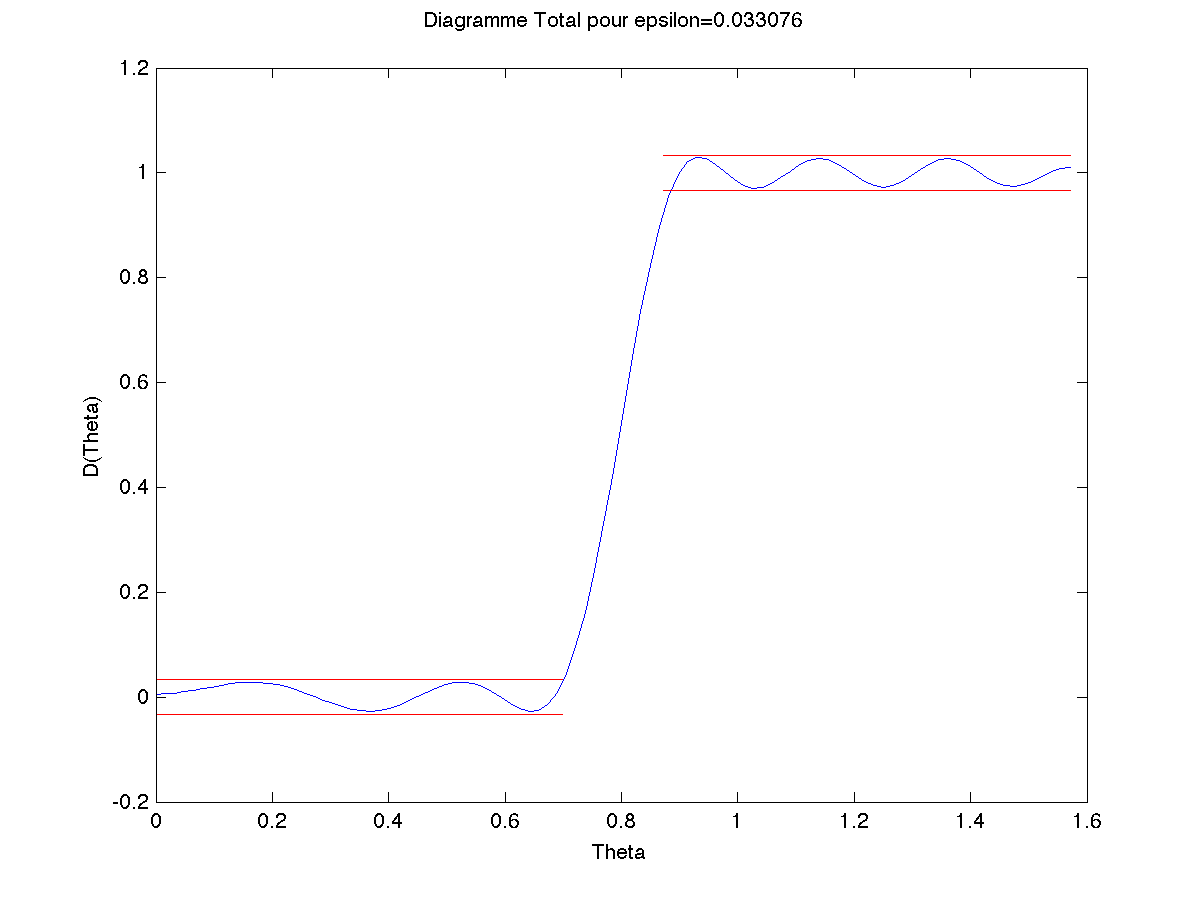
\includegraphics[width=\textwidth]{D-ModRobust1-01.png}
  \caption{$D(\theta)$ pour $\tau = 0.01$ et $x$ non-perturbé.}
  \label{fig:D-ModRobust1-01}
  \end{subfigure}%
  ~ 
 \begin{subfigure}[b]{0.45\textwidth}
  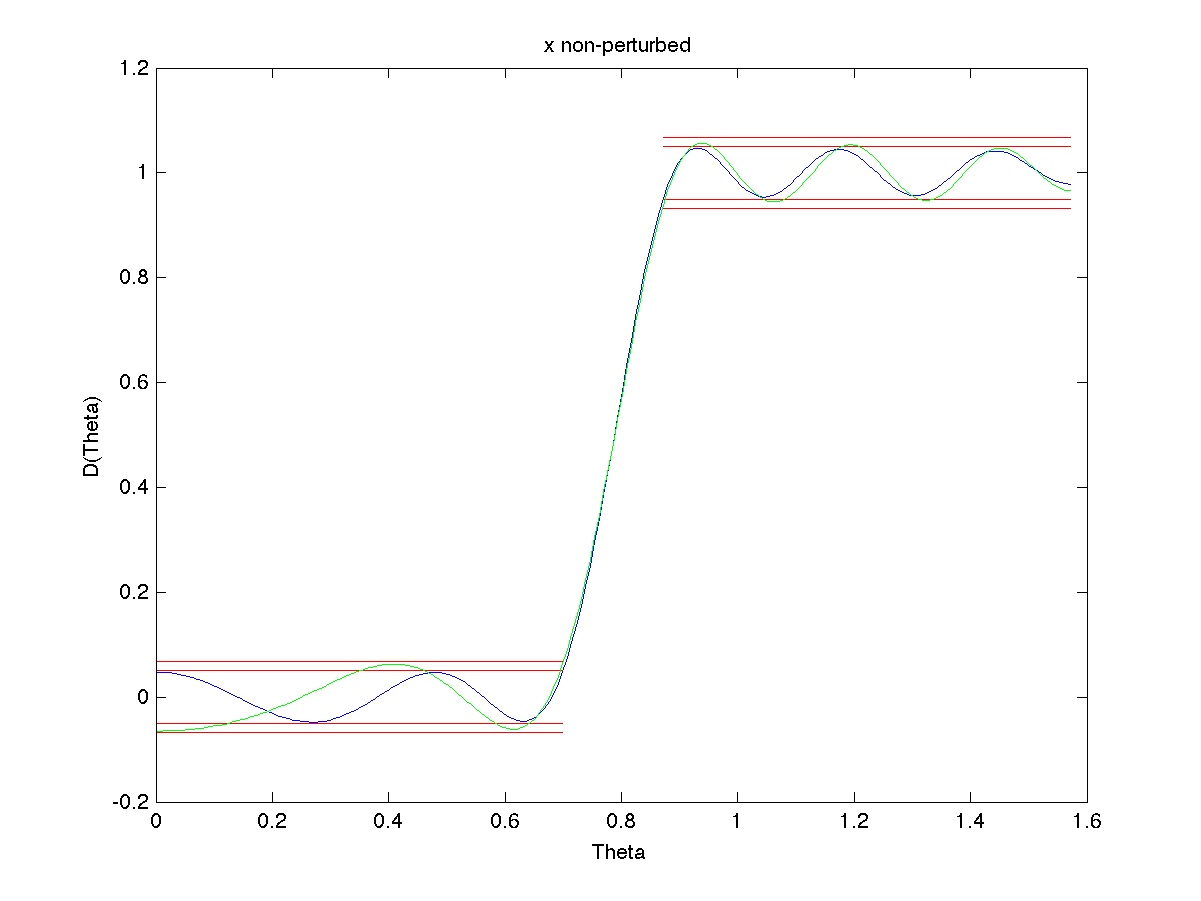
\includegraphics[width=\textwidth]{D-ModRobust1-001.png}
  \caption{$D(\theta)$ pour $\tau = 0.001$ et $x$ non-perturbé.}
  \label{fig:D-ModRobust1-001}
  \end{subfigure}
 \begin{subfigure}[b]{0.45\textwidth}
  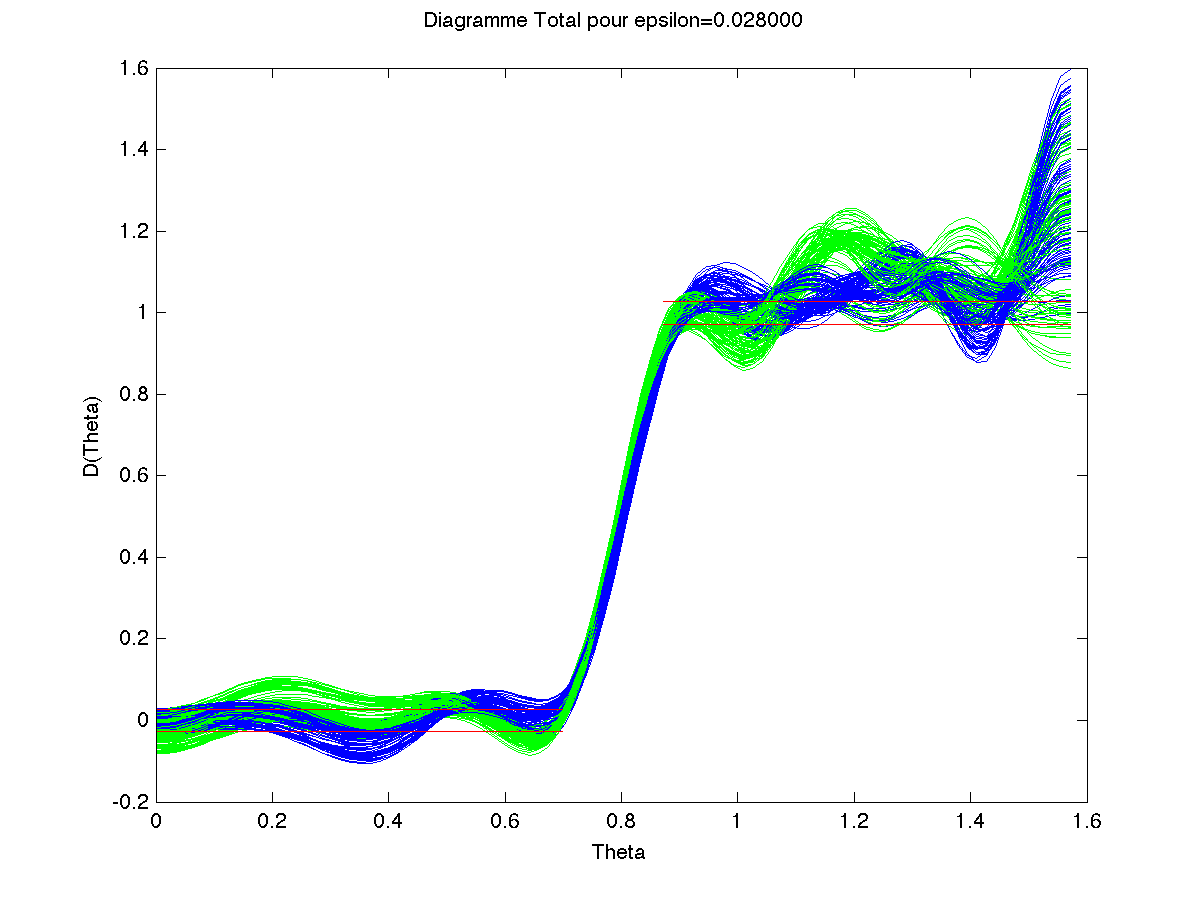
\includegraphics[width=\textwidth]{D-ModRobust1-test3RobTau001.png}
  \caption{$D(\theta)$ pour une perturbation de $\tau = 0.001$ et $x$ perturbés (en vert pour un modèle de $\tau=0.001$ en bleu pour $\tau=0.01$).}
  \label{fig:D-ModRobust1-test3RobTau001}
  \end{subfigure}%
  ~ 
  \begin{subfigure}[b]{0.45\textwidth}
  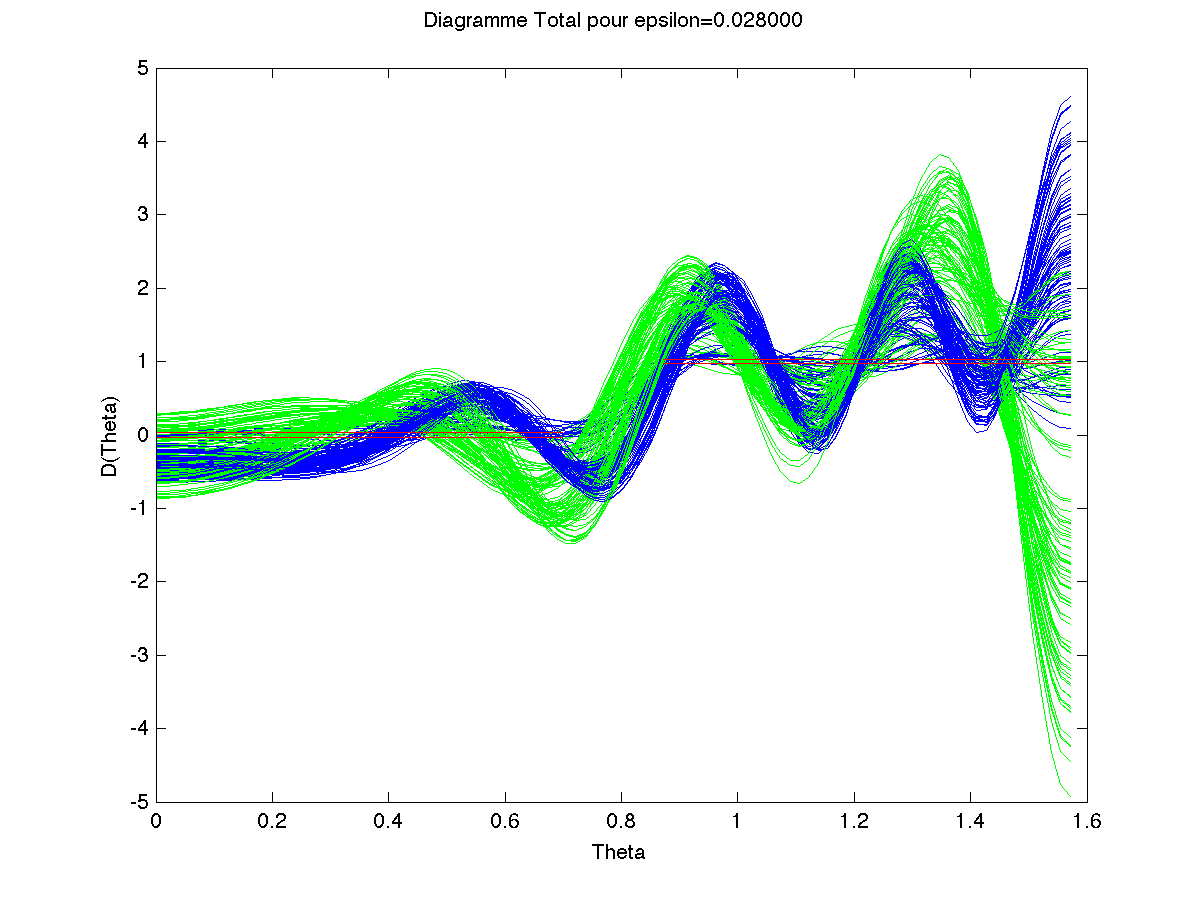
\includegraphics[width=\textwidth]{D-ModRobust1-test3RobTau01.png}
  \caption{$D(\theta)$ pour une perturbation de $\tau = 0.01$ et $x$ perturbés (en vert pour un modèle de $\tau=0.001$ en bleu pour $\tau=0.01$).}
  \label{fig:D-ModRobust1-test3RobTau01}
  \end{subfigure}
  \caption{}
  \end{figure}

\begin{table}
\centering
\begin{tabular}{c|c|ccc}
 & & & \textbf{Erreurs pour : } &\\
 & $\epsilon$ & $x_i$ non-perturbés & $x_i$ perturbés ($\tau=0.001$) & $x_i$ perturbés ($\tau=0.01$) \\
 \hline
Modèle de base & $2\%$ & 0.0185 & 5.3977 & 47.9054 \\
Modèle robuste 1 ($\tau=0.001$) & $2.8 \%$ & 0.0249 & 0.1315   & 0.9614 \\
Modèle robuste 1 ($\tau=0.01$)  & $3.3 \%$ & 0.0246 & 0.0564 & 0.7847 \\
\end{tabular}
\caption{Récapitulatif des résultats des erreurs et de la borne maximal $\epsilon$ obtenus pour les différents modèles et les différents types de perturbations.}
\label{table:Recap}
\end{table}